\documentclass[twoside]{book}

% Packages required by doxygen
\usepackage{fixltx2e}
\usepackage{calc}
\usepackage{doxygen}
\usepackage[export]{adjustbox} % also loads graphicx
\usepackage{graphicx}
\usepackage[utf8]{inputenc}
\usepackage{makeidx}
\usepackage{multicol}
\usepackage{multirow}
\PassOptionsToPackage{warn}{textcomp}
\usepackage{textcomp}
\usepackage[nointegrals]{wasysym}
\usepackage[table]{xcolor}

% Font selection
\usepackage[T1]{fontenc}
\usepackage[scaled=.90]{helvet}
\usepackage{courier}
\usepackage{amssymb}
\usepackage{sectsty}
\renewcommand{\familydefault}{\sfdefault}
\allsectionsfont{%
  \fontseries{bc}\selectfont%
  \color{darkgray}%
}
\renewcommand{\DoxyLabelFont}{%
  \fontseries{bc}\selectfont%
  \color{darkgray}%
}
\newcommand{\+}{\discretionary{\mbox{\scriptsize$\hookleftarrow$}}{}{}}

% Page & text layout
\usepackage{geometry}
\geometry{%
  a4paper,%
  top=2.5cm,%
  bottom=2.5cm,%
  left=2.5cm,%
  right=2.5cm%
}
\tolerance=750
\hfuzz=15pt
\hbadness=750
\setlength{\emergencystretch}{15pt}
\setlength{\parindent}{0cm}
\setlength{\parskip}{3ex plus 2ex minus 2ex}
\makeatletter
\renewcommand{\paragraph}{%
  \@startsection{paragraph}{4}{0ex}{-1.0ex}{1.0ex}{%
    \normalfont\normalsize\bfseries\SS@parafont%
  }%
}
\renewcommand{\subparagraph}{%
  \@startsection{subparagraph}{5}{0ex}{-1.0ex}{1.0ex}{%
    \normalfont\normalsize\bfseries\SS@subparafont%
  }%
}
\makeatother

% Headers & footers
\usepackage{fancyhdr}
\pagestyle{fancyplain}
\fancyhead[LE]{\fancyplain{}{\bfseries\thepage}}
\fancyhead[CE]{\fancyplain{}{}}
\fancyhead[RE]{\fancyplain{}{\bfseries\leftmark}}
\fancyhead[LO]{\fancyplain{}{\bfseries\rightmark}}
\fancyhead[CO]{\fancyplain{}{}}
\fancyhead[RO]{\fancyplain{}{\bfseries\thepage}}
\fancyfoot[LE]{\fancyplain{}{}}
\fancyfoot[CE]{\fancyplain{}{}}
\fancyfoot[RE]{\fancyplain{}{\bfseries\scriptsize Generated by Doxygen }}
\fancyfoot[LO]{\fancyplain{}{\bfseries\scriptsize Generated by Doxygen }}
\fancyfoot[CO]{\fancyplain{}{}}
\fancyfoot[RO]{\fancyplain{}{}}
\renewcommand{\footrulewidth}{0.4pt}
\renewcommand{\chaptermark}[1]{%
  \markboth{#1}{}%
}
\renewcommand{\sectionmark}[1]{%
  \markright{\thesection\ #1}%
}

% Indices & bibliography
\usepackage{natbib}
\usepackage[titles]{tocloft}
\setcounter{tocdepth}{3}
\setcounter{secnumdepth}{5}
\makeindex

% Hyperlinks (required, but should be loaded last)
\usepackage{ifpdf}
\ifpdf
  \usepackage[pdftex,pagebackref=true]{hyperref}
\else
  \usepackage[ps2pdf,pagebackref=true]{hyperref}
\fi
\hypersetup{%
  colorlinks=true,%
  linkcolor=blue,%
  citecolor=blue,%
  unicode%
}

% Custom commands
\newcommand{\clearemptydoublepage}{%
  \newpage{\pagestyle{empty}\cleardoublepage}%
}

\usepackage{caption}
\captionsetup{labelsep=space,justification=centering,font={bf},singlelinecheck=off,skip=4pt,position=top}

%===== C O N T E N T S =====

\begin{document}

% Titlepage & ToC
\hypersetup{pageanchor=false,
             bookmarksnumbered=true,
             pdfencoding=unicode
            }
\pagenumbering{alph}
\begin{titlepage}
\vspace*{7cm}
\begin{center}%
{\Large T\+S\+IP Decoder }\\
\vspace*{1cm}
{\large Generated by Doxygen 1.8.13}\\
\end{center}
\end{titlepage}
\clearemptydoublepage
\pagenumbering{roman}
\tableofcontents
\clearemptydoublepage
\pagenumbering{arabic}
\hypersetup{pageanchor=true}

%--- Begin generated contents ---
\chapter{T\+S\+IP Decoder}
\label{index}\hypertarget{index}{}\hypertarget{index_intro_sec}{}\section{Introduction}\label{index_intro_sec}
This program is designed to read and decode T\+S\+IP data packets.\hypertarget{index_install_sec}{}\section{Installation}\label{index_install_sec}
Both .pro files to compile with QT and a simple Makefile are included. To compile the program simply run make from the main program directory.\hypertarget{index_Decoder}{}\section{Decoder}\label{index_Decoder}
The packet is decoded first. The decoding process removes the escape characters and maps the flags, marking the packet starting and ending points.


\begin{DoxyCodeInclude}
  \textcolor{keywordflow}{while} (i < *raw\_len) \{
    \textcolor{comment}{// check for DLE}
    \textcolor{keywordflow}{if} (raw[i] == \hyperlink{tsip__read_8h_add7018db64fb17dd1e4664b4494be0ee}{DLE}) \{
      \textcolor{comment}{// check if there are still bytes left in the buffer}
      \textcolor{keywordflow}{if} (i + 1 < *raw\_len) \{
        \textcolor{comment}{// check the byte after the DLE}
        i++;
        \textcolor{keywordflow}{switch} (raw[i]) \{
        \textcolor{keywordflow}{case} \hyperlink{tsip__read_8h_af02558e983dd26832a852bf186ed6726}{ETX}:
          \textcolor{comment}{// end of packet}
          flag[*flag\_count] = *processed\_len;
          flag\_type[*flag\_count] = \hyperlink{tsip__decode_8h_aaadb960acba914ffc497ac7b256cdd55a5ed0c9e4189b86c84f9ded0501e9dd18}{end\_flag};
          (*flag\_count)++;
          \textcolor{keywordflow}{break};
        \textcolor{keywordflow}{case} \hyperlink{tsip__read_8h_add7018db64fb17dd1e4664b4494be0ee}{DLE}:
          \textcolor{comment}{// escape flag, don't do anything}
          processed[(*processed\_len)++] = raw[i];
          \textcolor{keywordflow}{break};
        \textcolor{keywordflow}{default}:
          \textcolor{comment}{// data start}
          flag[*flag\_count] = *processed\_len;
          flag\_type[*flag\_count] = \hyperlink{tsip__decode_8h_aaadb960acba914ffc497ac7b256cdd55a4b507f9b9a7feb19dc7248d7de612717}{start\_flag};
          (*flag\_count)++;
          processed[(*processed\_len)++] = raw[i];
          \textcolor{keywordflow}{break};
        \}
        i++;
      \} \textcolor{keywordflow}{else} \{
        \textcolor{comment}{// end of raw data, just store it as-is and figure it out}
        \textcolor{comment}{// later}
        *hanging\_dle = \textcolor{keyword}{true};
        processed[(*processed\_len)++] = raw[i];
        i++;
      \}
    \} \textcolor{keywordflow}{else} \{
      processed[(*processed\_len)++] = raw[i];
      i++;
    \}
  \}
\end{DoxyCodeInclude}
 Once the data block is processed, the previous data buffer is checked. This is done to ensure that if a packet is spread across several blocks it is still identified and parsed.


\begin{DoxyCodeInclude}
      \textcolor{comment}{// check if the last block ended on a DLE flag}
      \hyperlink{tsip__decode_8h_a812dd629379f16c30e1dba03db6745fc}{hanging\_dle\_test}(processed, processed\_len, flag, flag\_type, flag\_count);
      \textcolor{comment}{// make sure there are some flags found}
      \textcolor{keywordflow}{if} ((*flag\_count) > 0) \{
        \textcolor{comment}{// check if there's data from before}
        \textcolor{keywordflow}{if} (g\_inter\_buffer\_len > 0) \{

          \textcolor{keywordflow}{if} (flag\_type[0] == \hyperlink{tsip__decode_8h_aaadb960acba914ffc497ac7b256cdd55a5ed0c9e4189b86c84f9ded0501e9dd18}{end\_flag}) \{
            \textcolor{comment}{// patch the data together}
            memcpy(g\_inter\_buffer + g\_inter\_buffer\_len, processed,
                   flag[0] * \textcolor{keyword}{sizeof}(uint8\_t));
            g\_inter\_buffer\_len += flag[0];
            \textcolor{comment}{// validate and parse}
            \textcolor{keywordflow}{if} (\hyperlink{tsip__decode_8h_a41c4ae0abb32c8c722925578007e711b}{validate\_packet}(g\_inter\_buffer, 0, g\_inter\_buffer\_len) == 0) \{
              \hyperlink{tsip__read_8h_aaf187111fc27885f025120a9bf69de0d}{ParseTsipData}(g\_inter\_buffer, g\_inter\_buffer\_len - 4);
              packet\_counter++;
            \}
            \textcolor{comment}{// reset buffer}
            g\_inter\_buffer\_len = 0;
            g\_inter\_buffer\_dle = \textcolor{keyword}{false};
          \}
        \}
\end{DoxyCodeInclude}
 If a complete packet is identified, it is validated and parsed. The validation includes checking that the packet size does not exceed minimum or maximum limits, that the first byte ID is legal and a C\+RC checksum comparison.


\begin{DoxyCodeInclude}
  \textcolor{comment}{// packet size}
  \textcolor{keywordflow}{if} (len < 6 || len > \hyperlink{tsip__decode_8h_a87f68e96fb938eddc39ad1f19d923a96}{MAX\_DATA\_SIZE} + 6) \{
    \textcolor{keywordflow}{return} \hyperlink{tsip__decode_8h_ac1accdfaf17cd8ccf452c605fa935233a06e8eebf569c66387fe7e38059ceed79}{size\_mismatch};
  \}
  \textcolor{comment}{// ID}
  \textcolor{keywordflow}{if} (buffer[start] == \hyperlink{tsip__read_8h_add7018db64fb17dd1e4664b4494be0ee}{DLE}) \{
    \textcolor{keywordflow}{return} \hyperlink{tsip__decode_8h_ac1accdfaf17cd8ccf452c605fa935233aa7c3ec9f75a85e0e38eb97a1d7bd7490}{illegal\_id};
  \}

  \textcolor{comment}{// chksum}
  uint32\_t chksum\_start = end - 4;
  uint32\_t chksum\_int = \hyperlink{util_8h_ad96587305bb46bd47c2069e0aafd6530}{arr\_to\_int}(buffer + chksum\_start, 4);
  uint32\_t chksum\_chk = \hyperlink{util_8h_aa1921745f0c9cd9f201d624ca86dc40b}{crc32}(buffer, start, chksum\_start);
  \textcolor{keywordflow}{if} (chksum\_int != chksum\_chk) \{
    \textcolor{keywordflow}{return} \hyperlink{tsip__decode_8h_ac1accdfaf17cd8ccf452c605fa935233a732565fcd9231ccc944acf3624b80300}{chksum\_mismatch};
  \}
\end{DoxyCodeInclude}
 If the packet is not correct, a flag indicating the failure mode is returned. After validating the packets that might have started in the previous block, the current block is scanned for packets, which are also validated and parsed.


\begin{DoxyCodeInclude}
        \textcolor{comment}{// check the uninterrupted packets}
        \textcolor{keywordflow}{for} (i = 0; i < (*flag\_count) - 1; i++) \{
          \textcolor{keywordflow}{if} (flag\_type[i] == \hyperlink{tsip__decode_8h_aaadb960acba914ffc497ac7b256cdd55a4b507f9b9a7feb19dc7248d7de612717}{start\_flag} && flag\_type[i + 1] == 
      \hyperlink{tsip__decode_8h_aaadb960acba914ffc497ac7b256cdd55a5ed0c9e4189b86c84f9ded0501e9dd18}{end\_flag}) \{
            \textcolor{comment}{// uninterrupted packet, validate and parse}
            \textcolor{keywordflow}{if} (\hyperlink{tsip__decode_8h_a41c4ae0abb32c8c722925578007e711b}{validate\_packet}(processed, flag[i], flag[i + 1]) == 0) \{
              \hyperlink{tsip__read_8h_aaf187111fc27885f025120a9bf69de0d}{ParseTsipData}(processed + flag[i], flag[i + 1] - flag[i] - 4);
              packet\_counter++;
            \}
          \}
        \}
\end{DoxyCodeInclude}
 \hypertarget{index_Tests}{}\section{Tests}\label{index_Tests}
The tests included are the output and the speed tests. Two test data files are included in \char`\"{}data\char`\"{} folder\+: the tsip\+\_\+sample with 3 valid data blocks and the tsip\+\_\+sample\+\_\+ext with 30000 blocks.

The output test is run on the shorter block, while the timing test is run on the longer one. The shorter output test can be run by appending a binary filename as a program parameter for running extra tests.


\begin{DoxyCodeInclude}
  \textcolor{keywordflow}{if} (argc > 1) \{
    \textcolor{comment}{// load a provided file}
    \hyperlink{uavnav__main_8c_aad6066d9ede8cbf9b9d5e4fa28236380}{test\_data\_load}(argv[1]);
  \} \textcolor{keywordflow}{else} \{
    \textcolor{comment}{// or a default one if none provided}
    \hyperlink{uavnav__main_8c_aad6066d9ede8cbf9b9d5e4fa28236380}{test\_data\_load}(\textcolor{stringliteral}{"data/tsip\_sample"});
  \}
\end{DoxyCodeInclude}


The tests are run by executing the Task\+Uplink200\+Hz() command. This function starts the threads and keeps running until the entire data set is decoded.


\begin{DoxyCodeInclude}
  g\_data\_read\_seq = 0;
  \textcolor{keywordflow}{for} (uint8\_t i = 0; i < \hyperlink{tsip__decode_8h_ab60b5074c740fd36061f48f90d1a0b21}{N\_THREADS}; i++) \{
    ints[i] = i;
    pthread\_create(&thread[i], NULL, \hyperlink{tsip__decode_8h_a12e6599a2b96dd309e86e6fbb868a5d8}{extract\_data}, &ints[i]);
  \}
\end{DoxyCodeInclude}
 The example program output is shown below\+:

\begin{DoxyVerb}Running verbose test
Loaded file data/tsip_sample
Size: 135
ID1: 165 ID2: 9 CHKSUM: 0xe85817fd
56 96 8a f1
cb 6e 13 50
8f 3c 84 44
c1 03 7c fc
3e 00 db 04
1c 05 00 76
1d 10 00 ff
ff 00 00 00
00 00 00 00
00 b1 46 d6
43 20 4e

ID1: 165 ID2: 10 CHKSUM: 0xc4c61b3e
db 04 1c 05
f9 f6 6d 44
00 00 c5 0a
76 1d 10 00
20 4e

ID1: 57 ID2: 2 CHKSUM: 0x476753ec
64 61 3e 0f
c4 c6 8a 40


Decoded 3 packets

Running a timed test
Loaded file data/tsip_sample_ext
Size: 1350000
Decoded 29535 packets
Time taken 0 seconds 9 milliseconds
\end{DoxyVerb}


Note that the tsip\+\_\+sample\+\_\+ext file actually contains 30000 packet samples, so the program may still needs some improvements in that regard. The main problem comes from the fact that a single packet may span several blocks of data read from the C\+OM port, and separate blocks must be merged without losing data. Every possible condition must be taken into account. The decoder functionality and methods are described in the following section.

The verbose test shows that the packets are interpreted correctly. The timed test allows to compare the performance for different setup parameters, defined in advance.


\begin{DoxyCodeInclude}

\textcolor{preprocessor}{#define N\_THREADS 2}

\textcolor{preprocessor}{#define BLOCK\_SIZE 2048}

\textcolor{preprocessor}{#define MAX\_COM\_SIZE 512}

\textcolor{preprocessor}{#define MAX\_DATA\_SIZE 256}
\end{DoxyCodeInclude}
 The number of threads is defined by the variable N\+\_\+\+T\+H\+R\+E\+A\+DS. In theory spreading the load across several threads should increase the execution efficiency and reduce the execution times. In practice, a lot of this depends on the hardware architecture. On this machine (Intel(\+R) Core(\+T\+M) i7-\/3610\+QM C\+PU @ 2.\+30\+G\+Hz running Debian G\+N\+U/\+Linux) two threads performed slightly faster than a single thread, and the performance started to decrease once the number of threads exceeded 4. Among the disadvantages of a threaded approach is that it adds to complexity of the code, and any performance benefits of running separate threads could be negated by the demands of thread management itself.

The B\+L\+O\+C\+K\+\_\+\+S\+I\+ZE variable specifies the data block size to be processed by a single thread. It was found that larger block size results in a better performance. Which is natural, since it takes less effort to analyze one continuous data block rather than a series of discontinuous ones.

The M\+A\+X\+\_\+\+C\+O\+M\+\_\+\+S\+I\+ZE parameter is the maximum allowable data size that is allowed to read from the C\+OM port in one go. While the M\+A\+X\+\_\+\+D\+A\+T\+A\+\_\+\+S\+I\+ZE parameter is used to define the maximum packet size, and it is used for data validation and sanity checks. 
\chapter{uavnav\+\_\+tsip}
\label{md__r_e_a_d_m_e}
\Hypertarget{md__r_e_a_d_m_e}
A decoder for the T\+S\+IP protocol 
\chapter{File Index}
\section{File List}
Here is a list of all files with brief descriptions\+:\begin{DoxyCompactList}
\item\contentsline{section}{\hyperlink{tsip__decode_8h}{tsip\+\_\+decode.\+h} \\*Header containing the decoding functions. The main decoder code is contained here }{\pageref{tsip__decode_8h}}{}
\item\contentsline{section}{\hyperlink{tsip__read_8h}{tsip\+\_\+read.\+h} \\*Header containing the testing functions. These functions are designed to simulate the U\+AV parser and the C\+OM interface }{\pageref{tsip__read_8h}}{}
\item\contentsline{section}{\hyperlink{uavnav__main_8c}{uavnav\+\_\+main.\+c} \\*Main tester application. Loads the test data files, runs tests, outputs the }{\pageref{uavnav__main_8c}}{}
\item\contentsline{section}{\hyperlink{util_8h}{util.\+h} \\*Header containing the utility functions. Various utility functions, including the C\+RC checker }{\pageref{util_8h}}{}
\end{DoxyCompactList}

\chapter{File Documentation}
\hypertarget{_d_o_x_y_g_e_n___f_r_o_n_t_p_a_g_e_8md}{}\section{D\+O\+X\+Y\+G\+E\+N\+\_\+\+F\+R\+O\+N\+T\+P\+A\+G\+E.\+md File Reference}
\label{_d_o_x_y_g_e_n___f_r_o_n_t_p_a_g_e_8md}\index{D\+O\+X\+Y\+G\+E\+N\+\_\+\+F\+R\+O\+N\+T\+P\+A\+G\+E.\+md@{D\+O\+X\+Y\+G\+E\+N\+\_\+\+F\+R\+O\+N\+T\+P\+A\+G\+E.\+md}}

\hypertarget{_r_e_a_d_m_e_8md}{}\section{R\+E\+A\+D\+M\+E.\+md File Reference}
\label{_r_e_a_d_m_e_8md}\index{R\+E\+A\+D\+M\+E.\+md@{R\+E\+A\+D\+M\+E.\+md}}

\hypertarget{tsip__decode_8h}{}\section{tsip\+\_\+decode.\+h File Reference}
\label{tsip__decode_8h}\index{tsip\+\_\+decode.\+h@{tsip\+\_\+decode.\+h}}


Header containing the decoding functions. The main decoder code is contained here.  


{\ttfamily \#include \char`\"{}string.\+h\char`\"{}}\newline
{\ttfamily \#include $<$pthread.\+h$>$}\newline
{\ttfamily \#include $<$stdbool.\+h$>$}\newline
{\ttfamily \#include $<$stdint.\+h$>$}\newline
{\ttfamily \#include \char`\"{}tsip\+\_\+read.\+h\char`\"{}}\newline
Include dependency graph for tsip\+\_\+decode.\+h\+:\nopagebreak
\begin{figure}[H]
\begin{center}
\leavevmode
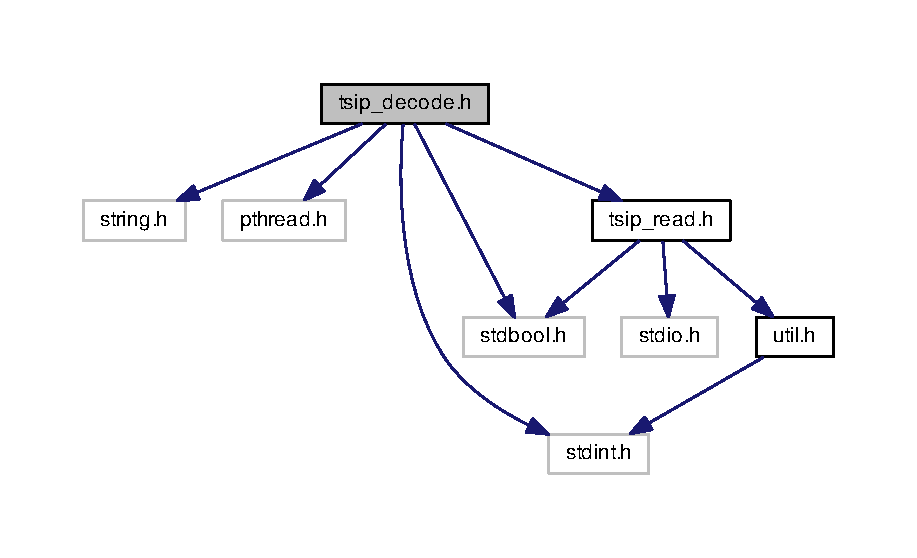
\includegraphics[width=350pt]{tsip__decode_8h__incl}
\end{center}
\end{figure}
This graph shows which files directly or indirectly include this file\+:\nopagebreak
\begin{figure}[H]
\begin{center}
\leavevmode
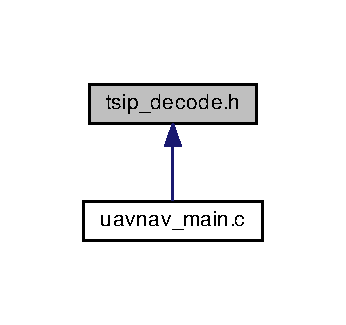
\includegraphics[width=166pt]{tsip__decode_8h__dep__incl}
\end{center}
\end{figure}
\subsection*{Macros}
\begin{DoxyCompactItemize}
\item 
\#define \hyperlink{tsip__decode_8h_ab60b5074c740fd36061f48f90d1a0b21}{N\+\_\+\+T\+H\+R\+E\+A\+DS}~2
\begin{DoxyCompactList}\small\item\em \mbox{[}Setup parameters\mbox{]} \end{DoxyCompactList}\item 
\#define \hyperlink{tsip__decode_8h_ad51ded0bbd705f02f73fc60c0b721ced}{B\+L\+O\+C\+K\+\_\+\+S\+I\+ZE}~2048
\begin{DoxyCompactList}\small\item\em Data block size to be processed by a single thread. \end{DoxyCompactList}\item 
\#define \hyperlink{tsip__decode_8h_a1a11ffedda6862cc09621931092dbaf5}{M\+A\+X\+\_\+\+C\+O\+M\+\_\+\+S\+I\+ZE}~512
\begin{DoxyCompactList}\small\item\em Maximum allowable raw data size. \end{DoxyCompactList}\item 
\#define \hyperlink{tsip__decode_8h_a87f68e96fb938eddc39ad1f19d923a96}{M\+A\+X\+\_\+\+D\+A\+T\+A\+\_\+\+S\+I\+ZE}~256
\begin{DoxyCompactList}\small\item\em Maximum allowable decoded data size. \end{DoxyCompactList}\item 
\#define \hyperlink{tsip__decode_8h_ad72dbcf6d0153db1b8d8a58001feed83}{D\+E\+B\+UG}~false
\begin{DoxyCompactList}\small\item\em \mbox{[}Setup parameters\mbox{]} \end{DoxyCompactList}\end{DoxyCompactItemize}
\subsection*{Enumerations}
\begin{DoxyCompactItemize}
\item 
enum \hyperlink{tsip__decode_8h_ac1accdfaf17cd8ccf452c605fa935233}{validate\+\_\+error} \{ \hyperlink{tsip__decode_8h_ac1accdfaf17cd8ccf452c605fa935233ab7e4e0120a041dbe6528b050c04269e0}{none}, 
\hyperlink{tsip__decode_8h_ac1accdfaf17cd8ccf452c605fa935233a06e8eebf569c66387fe7e38059ceed79}{size\+\_\+mismatch}, 
\hyperlink{tsip__decode_8h_ac1accdfaf17cd8ccf452c605fa935233aa7c3ec9f75a85e0e38eb97a1d7bd7490}{illegal\+\_\+id}, 
\hyperlink{tsip__decode_8h_ac1accdfaf17cd8ccf452c605fa935233a732565fcd9231ccc944acf3624b80300}{chksum\+\_\+mismatch}
 \}\begin{DoxyCompactList}\small\item\em Validation error types. \end{DoxyCompactList}
\item 
enum \hyperlink{tsip__decode_8h_aaadb960acba914ffc497ac7b256cdd55}{flag\+\_\+type\+\_\+enum} \{ \hyperlink{tsip__decode_8h_aaadb960acba914ffc497ac7b256cdd55a4b507f9b9a7feb19dc7248d7de612717}{start\+\_\+flag}, 
\hyperlink{tsip__decode_8h_aaadb960acba914ffc497ac7b256cdd55a5ed0c9e4189b86c84f9ded0501e9dd18}{end\+\_\+flag}
 \}\begin{DoxyCompactList}\small\item\em Special character flag types. \end{DoxyCompactList}
\end{DoxyCompactItemize}
\subsection*{Functions}
\begin{DoxyCompactItemize}
\item 
uint8\+\_\+t \hyperlink{tsip__decode_8h_a41c4ae0abb32c8c722925578007e711b}{validate\+\_\+packet} (const uint8\+\_\+t $\ast$buffer, const uint32\+\_\+t start, const uint32\+\_\+t end)
\begin{DoxyCompactList}\small\item\em Validate the packet. \end{DoxyCompactList}\item 
void \hyperlink{tsip__decode_8h_aa67c1cf61103414427db3eb35b74db60}{data\+\_\+read} (uint8\+\_\+t $\ast$raw, uint32\+\_\+t $\ast$raw\+\_\+len, uint8\+\_\+t id)
\begin{DoxyCompactList}\small\item\em Read the recieved raw data, multithread-\/protected. \end{DoxyCompactList}\item 
void \hyperlink{tsip__decode_8h_af38a027d040fb45e1614b59144351d34}{packet\+\_\+decode} (uint8\+\_\+t $\ast$processed, uint32\+\_\+t $\ast$processed\+\_\+len, uint8\+\_\+t $\ast$raw, uint32\+\_\+t $\ast$raw\+\_\+len, uint32\+\_\+t $\ast$flag, uint8\+\_\+t $\ast$flag\+\_\+type, uint32\+\_\+t $\ast$flag\+\_\+count, bool $\ast$hanging\+\_\+dle)
\begin{DoxyCompactList}\small\item\em Process raw data. \end{DoxyCompactList}\item 
void \hyperlink{tsip__decode_8h_a812dd629379f16c30e1dba03db6745fc}{hanging\+\_\+dle\+\_\+test} (uint8\+\_\+t $\ast$processed, uint32\+\_\+t processed\+\_\+len, uint32\+\_\+t $\ast$flag, uint8\+\_\+t $\ast$flag\+\_\+type, uint32\+\_\+t $\ast$flag\+\_\+count)
\begin{DoxyCompactList}\small\item\em Test for special condition that the previous block ended on a D\+LE. \end{DoxyCompactList}\item 
void \hyperlink{tsip__decode_8h_af34dd84879b0a89a108bcdce9cd5b20b}{trailing\+\_\+data\+\_\+store} (uint8\+\_\+t $\ast$processed, uint32\+\_\+t processed\+\_\+len, uint32\+\_\+t $\ast$flag, uint8\+\_\+t $\ast$flag\+\_\+type, uint32\+\_\+t $\ast$flag\+\_\+count, bool hanging\+\_\+dle)
\begin{DoxyCompactList}\small\item\em Store the trailing data. \end{DoxyCompactList}\item 
void \hyperlink{tsip__decode_8h_a2b9f28f133c97a87d0aa0ee8b1ba82fe}{data\+\_\+parse} (uint8\+\_\+t $\ast$processed, uint32\+\_\+t processed\+\_\+len, uint32\+\_\+t $\ast$flag, uint8\+\_\+t $\ast$flag\+\_\+type, uint32\+\_\+t $\ast$flag\+\_\+count, uint8\+\_\+t id, bool hanging\+\_\+dle)
\begin{DoxyCompactList}\small\item\em Parse the decoded data, multithread-\/protected. \end{DoxyCompactList}\item 
void $\ast$ \hyperlink{tsip__decode_8h_a12e6599a2b96dd309e86e6fbb868a5d8}{extract\+\_\+data} (void $\ast$tid)
\begin{DoxyCompactList}\small\item\em Data processing thread function. \end{DoxyCompactList}\item 
void \hyperlink{tsip__decode_8h_a15f61d2ad114da50125b6b5816a52a3d}{Task\+Up\+Link200\+Hz} ()
\begin{DoxyCompactList}\small\item\em Decoder task periodic function. \end{DoxyCompactList}\end{DoxyCompactItemize}


\subsection{Detailed Description}
Header containing the decoding functions. The main decoder code is contained here. 



\subsection{Macro Definition Documentation}
\mbox{\Hypertarget{tsip__decode_8h_ad51ded0bbd705f02f73fc60c0b721ced}\label{tsip__decode_8h_ad51ded0bbd705f02f73fc60c0b721ced}} 
\index{tsip\+\_\+decode.\+h@{tsip\+\_\+decode.\+h}!B\+L\+O\+C\+K\+\_\+\+S\+I\+ZE@{B\+L\+O\+C\+K\+\_\+\+S\+I\+ZE}}
\index{B\+L\+O\+C\+K\+\_\+\+S\+I\+ZE@{B\+L\+O\+C\+K\+\_\+\+S\+I\+ZE}!tsip\+\_\+decode.\+h@{tsip\+\_\+decode.\+h}}
\subsubsection{\texorpdfstring{B\+L\+O\+C\+K\+\_\+\+S\+I\+ZE}{BLOCK\_SIZE}}
{\footnotesize\ttfamily \#define B\+L\+O\+C\+K\+\_\+\+S\+I\+ZE~2048}



Data block size to be processed by a single thread. 

\mbox{\Hypertarget{tsip__decode_8h_ad72dbcf6d0153db1b8d8a58001feed83}\label{tsip__decode_8h_ad72dbcf6d0153db1b8d8a58001feed83}} 
\index{tsip\+\_\+decode.\+h@{tsip\+\_\+decode.\+h}!D\+E\+B\+UG@{D\+E\+B\+UG}}
\index{D\+E\+B\+UG@{D\+E\+B\+UG}!tsip\+\_\+decode.\+h@{tsip\+\_\+decode.\+h}}
\subsubsection{\texorpdfstring{D\+E\+B\+UG}{DEBUG}}
{\footnotesize\ttfamily \#define D\+E\+B\+UG~false}



\mbox{[}Setup parameters\mbox{]} 

Debug flag. \mbox{\Hypertarget{tsip__decode_8h_a1a11ffedda6862cc09621931092dbaf5}\label{tsip__decode_8h_a1a11ffedda6862cc09621931092dbaf5}} 
\index{tsip\+\_\+decode.\+h@{tsip\+\_\+decode.\+h}!M\+A\+X\+\_\+\+C\+O\+M\+\_\+\+S\+I\+ZE@{M\+A\+X\+\_\+\+C\+O\+M\+\_\+\+S\+I\+ZE}}
\index{M\+A\+X\+\_\+\+C\+O\+M\+\_\+\+S\+I\+ZE@{M\+A\+X\+\_\+\+C\+O\+M\+\_\+\+S\+I\+ZE}!tsip\+\_\+decode.\+h@{tsip\+\_\+decode.\+h}}
\subsubsection{\texorpdfstring{M\+A\+X\+\_\+\+C\+O\+M\+\_\+\+S\+I\+ZE}{MAX\_COM\_SIZE}}
{\footnotesize\ttfamily \#define M\+A\+X\+\_\+\+C\+O\+M\+\_\+\+S\+I\+ZE~512}



Maximum allowable raw data size. 

\mbox{\Hypertarget{tsip__decode_8h_a87f68e96fb938eddc39ad1f19d923a96}\label{tsip__decode_8h_a87f68e96fb938eddc39ad1f19d923a96}} 
\index{tsip\+\_\+decode.\+h@{tsip\+\_\+decode.\+h}!M\+A\+X\+\_\+\+D\+A\+T\+A\+\_\+\+S\+I\+ZE@{M\+A\+X\+\_\+\+D\+A\+T\+A\+\_\+\+S\+I\+ZE}}
\index{M\+A\+X\+\_\+\+D\+A\+T\+A\+\_\+\+S\+I\+ZE@{M\+A\+X\+\_\+\+D\+A\+T\+A\+\_\+\+S\+I\+ZE}!tsip\+\_\+decode.\+h@{tsip\+\_\+decode.\+h}}
\subsubsection{\texorpdfstring{M\+A\+X\+\_\+\+D\+A\+T\+A\+\_\+\+S\+I\+ZE}{MAX\_DATA\_SIZE}}
{\footnotesize\ttfamily \#define M\+A\+X\+\_\+\+D\+A\+T\+A\+\_\+\+S\+I\+ZE~256}



Maximum allowable decoded data size. 

\mbox{\Hypertarget{tsip__decode_8h_ab60b5074c740fd36061f48f90d1a0b21}\label{tsip__decode_8h_ab60b5074c740fd36061f48f90d1a0b21}} 
\index{tsip\+\_\+decode.\+h@{tsip\+\_\+decode.\+h}!N\+\_\+\+T\+H\+R\+E\+A\+DS@{N\+\_\+\+T\+H\+R\+E\+A\+DS}}
\index{N\+\_\+\+T\+H\+R\+E\+A\+DS@{N\+\_\+\+T\+H\+R\+E\+A\+DS}!tsip\+\_\+decode.\+h@{tsip\+\_\+decode.\+h}}
\subsubsection{\texorpdfstring{N\+\_\+\+T\+H\+R\+E\+A\+DS}{N\_THREADS}}
{\footnotesize\ttfamily \#define N\+\_\+\+T\+H\+R\+E\+A\+DS~2}



\mbox{[}Setup parameters\mbox{]} 

Number of concurrent threads. 

\subsection{Enumeration Type Documentation}
\mbox{\Hypertarget{tsip__decode_8h_aaadb960acba914ffc497ac7b256cdd55}\label{tsip__decode_8h_aaadb960acba914ffc497ac7b256cdd55}} 
\index{tsip\+\_\+decode.\+h@{tsip\+\_\+decode.\+h}!flag\+\_\+type\+\_\+enum@{flag\+\_\+type\+\_\+enum}}
\index{flag\+\_\+type\+\_\+enum@{flag\+\_\+type\+\_\+enum}!tsip\+\_\+decode.\+h@{tsip\+\_\+decode.\+h}}
\subsubsection{\texorpdfstring{flag\+\_\+type\+\_\+enum}{flag\_type\_enum}}
{\footnotesize\ttfamily enum \hyperlink{tsip__decode_8h_aaadb960acba914ffc497ac7b256cdd55}{flag\+\_\+type\+\_\+enum}}



Special character flag types. 

\begin{DoxyEnumFields}{Enumerator}
\raisebox{\heightof{T}}[0pt][0pt]{\index{start\+\_\+flag@{start\+\_\+flag}!tsip\+\_\+decode.\+h@{tsip\+\_\+decode.\+h}}\index{tsip\+\_\+decode.\+h@{tsip\+\_\+decode.\+h}!start\+\_\+flag@{start\+\_\+flag}}}\mbox{\Hypertarget{tsip__decode_8h_aaadb960acba914ffc497ac7b256cdd55a4b507f9b9a7feb19dc7248d7de612717}\label{tsip__decode_8h_aaadb960acba914ffc497ac7b256cdd55a4b507f9b9a7feb19dc7248d7de612717}} 
start\+\_\+flag&\\
\hline

\raisebox{\heightof{T}}[0pt][0pt]{\index{end\+\_\+flag@{end\+\_\+flag}!tsip\+\_\+decode.\+h@{tsip\+\_\+decode.\+h}}\index{tsip\+\_\+decode.\+h@{tsip\+\_\+decode.\+h}!end\+\_\+flag@{end\+\_\+flag}}}\mbox{\Hypertarget{tsip__decode_8h_aaadb960acba914ffc497ac7b256cdd55a5ed0c9e4189b86c84f9ded0501e9dd18}\label{tsip__decode_8h_aaadb960acba914ffc497ac7b256cdd55a5ed0c9e4189b86c84f9ded0501e9dd18}} 
end\+\_\+flag&\\
\hline

\end{DoxyEnumFields}
\mbox{\Hypertarget{tsip__decode_8h_ac1accdfaf17cd8ccf452c605fa935233}\label{tsip__decode_8h_ac1accdfaf17cd8ccf452c605fa935233}} 
\index{tsip\+\_\+decode.\+h@{tsip\+\_\+decode.\+h}!validate\+\_\+error@{validate\+\_\+error}}
\index{validate\+\_\+error@{validate\+\_\+error}!tsip\+\_\+decode.\+h@{tsip\+\_\+decode.\+h}}
\subsubsection{\texorpdfstring{validate\+\_\+error}{validate\_error}}
{\footnotesize\ttfamily enum \hyperlink{tsip__decode_8h_ac1accdfaf17cd8ccf452c605fa935233}{validate\+\_\+error}}



Validation error types. 

\begin{DoxyEnumFields}{Enumerator}
\raisebox{\heightof{T}}[0pt][0pt]{\index{none@{none}!tsip\+\_\+decode.\+h@{tsip\+\_\+decode.\+h}}\index{tsip\+\_\+decode.\+h@{tsip\+\_\+decode.\+h}!none@{none}}}\mbox{\Hypertarget{tsip__decode_8h_ac1accdfaf17cd8ccf452c605fa935233ab7e4e0120a041dbe6528b050c04269e0}\label{tsip__decode_8h_ac1accdfaf17cd8ccf452c605fa935233ab7e4e0120a041dbe6528b050c04269e0}} 
none&\\
\hline

\raisebox{\heightof{T}}[0pt][0pt]{\index{size\+\_\+mismatch@{size\+\_\+mismatch}!tsip\+\_\+decode.\+h@{tsip\+\_\+decode.\+h}}\index{tsip\+\_\+decode.\+h@{tsip\+\_\+decode.\+h}!size\+\_\+mismatch@{size\+\_\+mismatch}}}\mbox{\Hypertarget{tsip__decode_8h_ac1accdfaf17cd8ccf452c605fa935233a06e8eebf569c66387fe7e38059ceed79}\label{tsip__decode_8h_ac1accdfaf17cd8ccf452c605fa935233a06e8eebf569c66387fe7e38059ceed79}} 
size\+\_\+mismatch&\\
\hline

\raisebox{\heightof{T}}[0pt][0pt]{\index{illegal\+\_\+id@{illegal\+\_\+id}!tsip\+\_\+decode.\+h@{tsip\+\_\+decode.\+h}}\index{tsip\+\_\+decode.\+h@{tsip\+\_\+decode.\+h}!illegal\+\_\+id@{illegal\+\_\+id}}}\mbox{\Hypertarget{tsip__decode_8h_ac1accdfaf17cd8ccf452c605fa935233aa7c3ec9f75a85e0e38eb97a1d7bd7490}\label{tsip__decode_8h_ac1accdfaf17cd8ccf452c605fa935233aa7c3ec9f75a85e0e38eb97a1d7bd7490}} 
illegal\+\_\+id&\\
\hline

\raisebox{\heightof{T}}[0pt][0pt]{\index{chksum\+\_\+mismatch@{chksum\+\_\+mismatch}!tsip\+\_\+decode.\+h@{tsip\+\_\+decode.\+h}}\index{tsip\+\_\+decode.\+h@{tsip\+\_\+decode.\+h}!chksum\+\_\+mismatch@{chksum\+\_\+mismatch}}}\mbox{\Hypertarget{tsip__decode_8h_ac1accdfaf17cd8ccf452c605fa935233a732565fcd9231ccc944acf3624b80300}\label{tsip__decode_8h_ac1accdfaf17cd8ccf452c605fa935233a732565fcd9231ccc944acf3624b80300}} 
chksum\+\_\+mismatch&\\
\hline

\end{DoxyEnumFields}


\subsection{Function Documentation}
\mbox{\Hypertarget{tsip__decode_8h_a2b9f28f133c97a87d0aa0ee8b1ba82fe}\label{tsip__decode_8h_a2b9f28f133c97a87d0aa0ee8b1ba82fe}} 
\index{tsip\+\_\+decode.\+h@{tsip\+\_\+decode.\+h}!data\+\_\+parse@{data\+\_\+parse}}
\index{data\+\_\+parse@{data\+\_\+parse}!tsip\+\_\+decode.\+h@{tsip\+\_\+decode.\+h}}
\subsubsection{\texorpdfstring{data\+\_\+parse()}{data\_parse()}}
{\footnotesize\ttfamily void data\+\_\+parse (\begin{DoxyParamCaption}\item[{uint8\+\_\+t $\ast$}]{processed,  }\item[{uint32\+\_\+t}]{processed\+\_\+len,  }\item[{uint32\+\_\+t $\ast$}]{flag,  }\item[{uint8\+\_\+t $\ast$}]{flag\+\_\+type,  }\item[{uint32\+\_\+t $\ast$}]{flag\+\_\+count,  }\item[{uint8\+\_\+t}]{id,  }\item[{bool}]{hanging\+\_\+dle }\end{DoxyParamCaption})}



Parse the decoded data, multithread-\/protected. 

Format the data, run the checks on the preceding data block. Run the validation checks. Parse the data if it\textquotesingle{}s correct. Store the trailing part that has not been parsed. Only one thread can parse the data at a time to make sure that it\textquotesingle{}s parsed in the same order as it comes in.


\begin{DoxyParams}[1]{Parameters}
\mbox{\tt in}  & {\em processed} & Pointer to processed data. \\
\hline
\mbox{\tt in}  & {\em processed\+\_\+len} & Size of processed data. \\
\hline
\mbox{\tt in}  & {\em flag} & Pointer to flags, contains flag locations. \\
\hline
\mbox{\tt in}  & {\em flag\+\_\+type} & Types of marked flags. \\
\hline
\mbox{\tt in}  & {\em flag\+\_\+count} & Number of flags. \\
\hline
\mbox{\tt in}  & {\em id} & Thread id. \\
\hline
\mbox{\tt in}  & {\em hanging\+\_\+dle} & Hanging D\+LE character indicator. \\
\hline
\end{DoxyParams}
\begin{DoxyReturn}{Returns}

\end{DoxyReturn}
\mbox{[}Checking previous buffer\mbox{]}

\mbox{[}Checking previous buffer\mbox{]}

\mbox{[}Checking uninterrupted packets\mbox{]}

\mbox{[}Checking uninterrupted packets\mbox{]} \mbox{\Hypertarget{tsip__decode_8h_aa67c1cf61103414427db3eb35b74db60}\label{tsip__decode_8h_aa67c1cf61103414427db3eb35b74db60}} 
\index{tsip\+\_\+decode.\+h@{tsip\+\_\+decode.\+h}!data\+\_\+read@{data\+\_\+read}}
\index{data\+\_\+read@{data\+\_\+read}!tsip\+\_\+decode.\+h@{tsip\+\_\+decode.\+h}}
\subsubsection{\texorpdfstring{data\+\_\+read()}{data\_read()}}
{\footnotesize\ttfamily void data\+\_\+read (\begin{DoxyParamCaption}\item[{uint8\+\_\+t $\ast$}]{raw,  }\item[{uint32\+\_\+t $\ast$}]{raw\+\_\+len,  }\item[{uint8\+\_\+t}]{id }\end{DoxyParamCaption})}



Read the recieved raw data, multithread-\/protected. 

Read the data. Only one thread is allowed to read data at a time.


\begin{DoxyParams}{Parameters}
{\em raw} & Pointer to raw data destination. \\
\hline
{\em raw\+\_\+len} & Pointer to the size of the data read. \\
\hline
{\em id} & Thread id. \\
\hline
\end{DoxyParams}
\begin{DoxyReturn}{Returns}
Error type, 0 if no errors are found. 
\end{DoxyReturn}
\mbox{[}Reading C\+OM data\mbox{]}

\mbox{[}Reading C\+OM data\mbox{]} \mbox{\Hypertarget{tsip__decode_8h_a12e6599a2b96dd309e86e6fbb868a5d8}\label{tsip__decode_8h_a12e6599a2b96dd309e86e6fbb868a5d8}} 
\index{tsip\+\_\+decode.\+h@{tsip\+\_\+decode.\+h}!extract\+\_\+data@{extract\+\_\+data}}
\index{extract\+\_\+data@{extract\+\_\+data}!tsip\+\_\+decode.\+h@{tsip\+\_\+decode.\+h}}
\subsubsection{\texorpdfstring{extract\+\_\+data()}{extract\_data()}}
{\footnotesize\ttfamily void$\ast$ extract\+\_\+data (\begin{DoxyParamCaption}\item[{void $\ast$}]{tid }\end{DoxyParamCaption})}



Data processing thread function. 

Thread function tasked with reading, decoding and parsing the data. Only one thread can read or parse the data at a time, while the decoding is done concurrently.


\begin{DoxyParams}[1]{Parameters}
\mbox{\tt in}  & {\em tid} & Thread id. \\
\hline
\end{DoxyParams}
\begin{DoxyReturn}{Returns}

\end{DoxyReturn}
\mbox{\Hypertarget{tsip__decode_8h_a812dd629379f16c30e1dba03db6745fc}\label{tsip__decode_8h_a812dd629379f16c30e1dba03db6745fc}} 
\index{tsip\+\_\+decode.\+h@{tsip\+\_\+decode.\+h}!hanging\+\_\+dle\+\_\+test@{hanging\+\_\+dle\+\_\+test}}
\index{hanging\+\_\+dle\+\_\+test@{hanging\+\_\+dle\+\_\+test}!tsip\+\_\+decode.\+h@{tsip\+\_\+decode.\+h}}
\subsubsection{\texorpdfstring{hanging\+\_\+dle\+\_\+test()}{hanging\_dle\_test()}}
{\footnotesize\ttfamily void hanging\+\_\+dle\+\_\+test (\begin{DoxyParamCaption}\item[{uint8\+\_\+t $\ast$}]{processed,  }\item[{uint32\+\_\+t}]{processed\+\_\+len,  }\item[{uint32\+\_\+t $\ast$}]{flag,  }\item[{uint8\+\_\+t $\ast$}]{flag\+\_\+type,  }\item[{uint32\+\_\+t $\ast$}]{flag\+\_\+count }\end{DoxyParamCaption})}



Test for special condition that the previous block ended on a D\+LE. 

Check if the previous raw data block ended on a D\+LE. Correct the following data block structure and data to match the trailing D\+LE character.


\begin{DoxyParams}[1]{Parameters}
\mbox{\tt in}  & {\em processed} & Pointer to processed data \\
\hline
\mbox{\tt in}  & {\em processed\+\_\+len} & Size of processed data \\
\hline
 & {\em flag} & Pointer to flags, contains flag locations \\
\hline
 & {\em flag\+\_\+type} & Types of marked flags \\
\hline
 & {\em flag\+\_\+count} & Number of flags \\
\hline
\end{DoxyParams}
\begin{DoxyReturn}{Returns}

\end{DoxyReturn}
\mbox{[}Checking hanging D\+LE flags\mbox{]}

\mbox{[}Checking hanging D\+LE flags\mbox{]} \mbox{\Hypertarget{tsip__decode_8h_af38a027d040fb45e1614b59144351d34}\label{tsip__decode_8h_af38a027d040fb45e1614b59144351d34}} 
\index{tsip\+\_\+decode.\+h@{tsip\+\_\+decode.\+h}!packet\+\_\+decode@{packet\+\_\+decode}}
\index{packet\+\_\+decode@{packet\+\_\+decode}!tsip\+\_\+decode.\+h@{tsip\+\_\+decode.\+h}}
\subsubsection{\texorpdfstring{packet\+\_\+decode()}{packet\_decode()}}
{\footnotesize\ttfamily void packet\+\_\+decode (\begin{DoxyParamCaption}\item[{uint8\+\_\+t $\ast$}]{processed,  }\item[{uint32\+\_\+t $\ast$}]{processed\+\_\+len,  }\item[{uint8\+\_\+t $\ast$}]{raw,  }\item[{uint32\+\_\+t $\ast$}]{raw\+\_\+len,  }\item[{uint32\+\_\+t $\ast$}]{flag,  }\item[{uint8\+\_\+t $\ast$}]{flag\+\_\+type,  }\item[{uint32\+\_\+t $\ast$}]{flag\+\_\+count,  }\item[{bool $\ast$}]{hanging\+\_\+dle }\end{DoxyParamCaption})}



Process raw data. 

Process the raw data, removing the escape characters and marking packet start and end points


\begin{DoxyParams}{Parameters}
{\em processed} & Pointer to destination. \\
\hline
{\em processed\+\_\+len} & Size of processed data. \\
\hline
{\em raw} & Pointer to source raw data. \\
\hline
{\em raw\+\_\+len} & Size of source data. \\
\hline
{\em flag} & Pointer to flags, contains flag locations. \\
\hline
{\em flag\+\_\+type} & Types of marked flags. \\
\hline
{\em flag\+\_\+count} & Number of flags. \\
\hline
{\em hanging\+\_\+dle} & A flag to indicate a hanging D\+LE character. \\
\hline
\end{DoxyParams}
\begin{DoxyReturn}{Returns}

\end{DoxyReturn}
\mbox{[}Removing escape characters\mbox{]}

\mbox{[}Removing escape characters\mbox{]} \mbox{\Hypertarget{tsip__decode_8h_a15f61d2ad114da50125b6b5816a52a3d}\label{tsip__decode_8h_a15f61d2ad114da50125b6b5816a52a3d}} 
\index{tsip\+\_\+decode.\+h@{tsip\+\_\+decode.\+h}!Task\+Up\+Link200\+Hz@{Task\+Up\+Link200\+Hz}}
\index{Task\+Up\+Link200\+Hz@{Task\+Up\+Link200\+Hz}!tsip\+\_\+decode.\+h@{tsip\+\_\+decode.\+h}}
\subsubsection{\texorpdfstring{Task\+Up\+Link200\+Hz()}{TaskUpLink200Hz()}}
{\footnotesize\ttfamily void Task\+Up\+Link200\+Hz (\begin{DoxyParamCaption}{ }\end{DoxyParamCaption})}



Decoder task periodic function. 

This function spawns several decoder threads

\begin{DoxyReturn}{Returns}

\end{DoxyReturn}
\mbox{[}Starting threads\mbox{]}

\mbox{[}Starting threads\mbox{]} \mbox{\Hypertarget{tsip__decode_8h_af34dd84879b0a89a108bcdce9cd5b20b}\label{tsip__decode_8h_af34dd84879b0a89a108bcdce9cd5b20b}} 
\index{tsip\+\_\+decode.\+h@{tsip\+\_\+decode.\+h}!trailing\+\_\+data\+\_\+store@{trailing\+\_\+data\+\_\+store}}
\index{trailing\+\_\+data\+\_\+store@{trailing\+\_\+data\+\_\+store}!tsip\+\_\+decode.\+h@{tsip\+\_\+decode.\+h}}
\subsubsection{\texorpdfstring{trailing\+\_\+data\+\_\+store()}{trailing\_data\_store()}}
{\footnotesize\ttfamily void trailing\+\_\+data\+\_\+store (\begin{DoxyParamCaption}\item[{uint8\+\_\+t $\ast$}]{processed,  }\item[{uint32\+\_\+t}]{processed\+\_\+len,  }\item[{uint32\+\_\+t $\ast$}]{flag,  }\item[{uint8\+\_\+t $\ast$}]{flag\+\_\+type,  }\item[{uint32\+\_\+t $\ast$}]{flag\+\_\+count,  }\item[{bool}]{hanging\+\_\+dle }\end{DoxyParamCaption})}



Store the trailing data. 

If no D\+L\+E/\+E\+TX combo is found at the end of the packet, pass on it\textquotesingle{}s trailing part to the next evaluation.


\begin{DoxyParams}[1]{Parameters}
\mbox{\tt in}  & {\em processed} & Pointer to processed data. \\
\hline
\mbox{\tt in}  & {\em processed\+\_\+len} & Size of processed data. \\
\hline
\mbox{\tt in}  & {\em flag} & Pointer to flags, contains flag locations. \\
\hline
\mbox{\tt in}  & {\em flag\+\_\+type} & Types of marked flags. \\
\hline
\mbox{\tt in}  & {\em flag\+\_\+count} & Number of flags. \\
\hline
\mbox{\tt in}  & {\em hanging\+\_\+dle} & Hanging D\+LE character indicator. \\
\hline
\end{DoxyParams}
\begin{DoxyReturn}{Returns}

\end{DoxyReturn}
\mbox{[}Storing trailing data\mbox{]}

\mbox{[}Storing trailing data\mbox{]} \mbox{\Hypertarget{tsip__decode_8h_a41c4ae0abb32c8c722925578007e711b}\label{tsip__decode_8h_a41c4ae0abb32c8c722925578007e711b}} 
\index{tsip\+\_\+decode.\+h@{tsip\+\_\+decode.\+h}!validate\+\_\+packet@{validate\+\_\+packet}}
\index{validate\+\_\+packet@{validate\+\_\+packet}!tsip\+\_\+decode.\+h@{tsip\+\_\+decode.\+h}}
\subsubsection{\texorpdfstring{validate\+\_\+packet()}{validate\_packet()}}
{\footnotesize\ttfamily uint8\+\_\+t validate\+\_\+packet (\begin{DoxyParamCaption}\item[{const uint8\+\_\+t $\ast$}]{buffer,  }\item[{const uint32\+\_\+t}]{start,  }\item[{const uint32\+\_\+t}]{end }\end{DoxyParamCaption})}



Validate the packet. 

Check the packet integrity, correct size and parameters. Run a C\+RC check.


\begin{DoxyParams}{Parameters}
{\em buffer} & Pointer to packet source. \\
\hline
{\em start} & Packet data start. \\
\hline
{\em end} & Packet data end. \\
\hline
\end{DoxyParams}
\begin{DoxyReturn}{Returns}
Error type, 0 if no errors are found. 
\end{DoxyReturn}
\mbox{[}Validating packet\mbox{]}

\mbox{[}Validating packet\mbox{]} 
\hypertarget{tsip__read_8h}{}\section{tsip\+\_\+read.\+h File Reference}
\label{tsip__read_8h}\index{tsip\+\_\+read.\+h@{tsip\+\_\+read.\+h}}


Header containing the testing functions. These functions are designed to simulate the U\+AV parser and the C\+OM interface.  


{\ttfamily \#include \char`\"{}stdio.\+h\char`\"{}}\newline
{\ttfamily \#include \char`\"{}util.\+h\char`\"{}}\newline
{\ttfamily \#include \char`\"{}stdbool.\+h\char`\"{}}\newline
Include dependency graph for tsip\+\_\+read.\+h\+:
\nopagebreak
\begin{figure}[H]
\begin{center}
\leavevmode
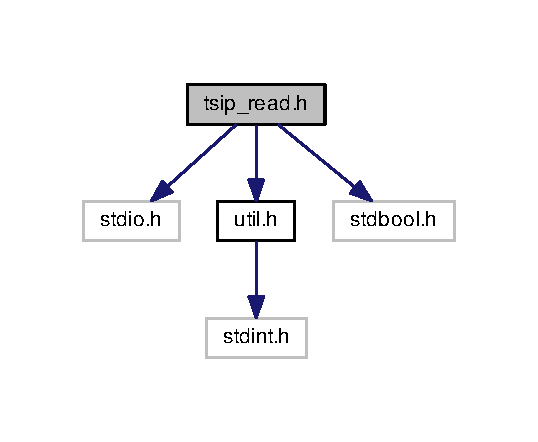
\includegraphics[width=258pt]{tsip__read_8h__incl}
\end{center}
\end{figure}
This graph shows which files directly or indirectly include this file\+:
\nopagebreak
\begin{figure}[H]
\begin{center}
\leavevmode
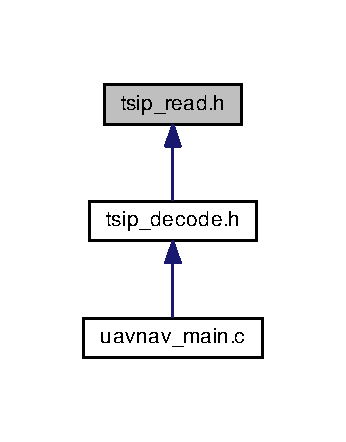
\includegraphics[width=166pt]{tsip__read_8h__dep__incl}
\end{center}
\end{figure}
\subsection*{Macros}
\begin{DoxyCompactItemize}
\item 
\#define \hyperlink{tsip__read_8h_add7018db64fb17dd1e4664b4494be0ee}{D\+LE}~0x10
\begin{DoxyCompactList}\small\item\em D\+LE flag. \end{DoxyCompactList}\item 
\#define \hyperlink{tsip__read_8h_af02558e983dd26832a852bf186ed6726}{E\+TX}~0x03
\begin{DoxyCompactList}\small\item\em E\+TX flag. \end{DoxyCompactList}\end{DoxyCompactItemize}
\subsection*{Functions}
\begin{DoxyCompactItemize}
\item 
uint32\+\_\+t \hyperlink{tsip__read_8h_ac21803ff4ef3330e13f027597975d26f}{uavn\+Com\+Read} (uint8\+\_\+t $\ast$const buffer, const uint32\+\_\+t count)
\begin{DoxyCompactList}\small\item\em Read received raw data from C\+OM port. \end{DoxyCompactList}\item 
void \hyperlink{tsip__read_8h_aaf187111fc27885f025120a9bf69de0d}{Parse\+Tsip\+Data} (const uint8\+\_\+t $\ast$const buffer, const uint32\+\_\+t number\+Of\+Bytes)
\begin{DoxyCompactList}\small\item\em Parse a T\+S\+IP data. \end{DoxyCompactList}\end{DoxyCompactItemize}
\subsection*{Variables}
\begin{DoxyCompactItemize}
\item 
unsigned char $\ast$ \hyperlink{tsip__read_8h_a5e287a26406318ae22f91b2186e093a1}{g\+\_\+test\+\_\+data}
\begin{DoxyCompactList}\small\item\em Test data array. \end{DoxyCompactList}\item 
uint32\+\_\+t \hyperlink{tsip__read_8h_aa0982aa6ad6c582eac44366139eec768}{g\+\_\+test\+\_\+data\+\_\+len}
\begin{DoxyCompactList}\small\item\em Test data length. \end{DoxyCompactList}\item 
uint32\+\_\+t \hyperlink{tsip__read_8h_af8a23b978deb1bf1c3e33bc838fecf69}{g\+\_\+test\+\_\+data\+\_\+start}
\begin{DoxyCompactList}\small\item\em Start of the test data. \end{DoxyCompactList}\item 
bool \hyperlink{tsip__read_8h_af8fbc191e3a97ad0427003b79f03144e}{g\+\_\+verbose\+\_\+output}
\begin{DoxyCompactList}\small\item\em Verbose output parameter. \end{DoxyCompactList}\end{DoxyCompactItemize}


\subsection{Detailed Description}
Header containing the testing functions. These functions are designed to simulate the U\+AV parser and the C\+OM interface. 



\subsection{Macro Definition Documentation}
\mbox{\Hypertarget{tsip__read_8h_add7018db64fb17dd1e4664b4494be0ee}\label{tsip__read_8h_add7018db64fb17dd1e4664b4494be0ee}} 
\index{tsip\+\_\+read.\+h@{tsip\+\_\+read.\+h}!D\+LE@{D\+LE}}
\index{D\+LE@{D\+LE}!tsip\+\_\+read.\+h@{tsip\+\_\+read.\+h}}
\subsubsection{\texorpdfstring{D\+LE}{DLE}}
{\footnotesize\ttfamily \#define D\+LE~0x10}



D\+LE flag. 

\mbox{\Hypertarget{tsip__read_8h_af02558e983dd26832a852bf186ed6726}\label{tsip__read_8h_af02558e983dd26832a852bf186ed6726}} 
\index{tsip\+\_\+read.\+h@{tsip\+\_\+read.\+h}!E\+TX@{E\+TX}}
\index{E\+TX@{E\+TX}!tsip\+\_\+read.\+h@{tsip\+\_\+read.\+h}}
\subsubsection{\texorpdfstring{E\+TX}{ETX}}
{\footnotesize\ttfamily \#define E\+TX~0x03}



E\+TX flag. 



\subsection{Function Documentation}
\mbox{\Hypertarget{tsip__read_8h_aaf187111fc27885f025120a9bf69de0d}\label{tsip__read_8h_aaf187111fc27885f025120a9bf69de0d}} 
\index{tsip\+\_\+read.\+h@{tsip\+\_\+read.\+h}!Parse\+Tsip\+Data@{Parse\+Tsip\+Data}}
\index{Parse\+Tsip\+Data@{Parse\+Tsip\+Data}!tsip\+\_\+read.\+h@{tsip\+\_\+read.\+h}}
\subsubsection{\texorpdfstring{Parse\+Tsip\+Data()}{ParseTsipData()}}
{\footnotesize\ttfamily void Parse\+Tsip\+Data (\begin{DoxyParamCaption}\item[{const uint8\+\_\+t $\ast$const}]{buffer,  }\item[{const uint32\+\_\+t}]{number\+Of\+Bytes }\end{DoxyParamCaption})}



Parse a T\+S\+IP data. 


\begin{DoxyParams}[1]{Parameters}
\mbox{\tt in}  & {\em buffer} & Const pointer where data is located. \\
\hline
\mbox{\tt in}  & {\em number\+Of\+Bytes} & It is filled with the number bytes in the T\+S\+IP packet. \\
\hline
\end{DoxyParams}
\mbox{\Hypertarget{tsip__read_8h_ac21803ff4ef3330e13f027597975d26f}\label{tsip__read_8h_ac21803ff4ef3330e13f027597975d26f}} 
\index{tsip\+\_\+read.\+h@{tsip\+\_\+read.\+h}!uavn\+Com\+Read@{uavn\+Com\+Read}}
\index{uavn\+Com\+Read@{uavn\+Com\+Read}!tsip\+\_\+read.\+h@{tsip\+\_\+read.\+h}}
\subsubsection{\texorpdfstring{uavn\+Com\+Read()}{uavnComRead()}}
{\footnotesize\ttfamily uint32\+\_\+t uavn\+Com\+Read (\begin{DoxyParamCaption}\item[{uint8\+\_\+t $\ast$const}]{buffer,  }\item[{const uint32\+\_\+t}]{count }\end{DoxyParamCaption})}



Read received raw data from C\+OM port. 

This is a non-\/blocking read function. This means that only available received data will be served. User may decide to call this function within a loop until the desired amount of data is received.


\begin{DoxyParams}{Parameters}
{\em buffer} & Pointer to destination buffer where to copy received data. \\
\hline
{\em count} & Maximum number of bytes to be read. \\
\hline
\end{DoxyParams}
\begin{DoxyReturn}{Returns}
Number of read bytes. This value will always be $<$= count. 
\end{DoxyReturn}


\subsection{Variable Documentation}
\mbox{\Hypertarget{tsip__read_8h_a5e287a26406318ae22f91b2186e093a1}\label{tsip__read_8h_a5e287a26406318ae22f91b2186e093a1}} 
\index{tsip\+\_\+read.\+h@{tsip\+\_\+read.\+h}!g\+\_\+test\+\_\+data@{g\+\_\+test\+\_\+data}}
\index{g\+\_\+test\+\_\+data@{g\+\_\+test\+\_\+data}!tsip\+\_\+read.\+h@{tsip\+\_\+read.\+h}}
\subsubsection{\texorpdfstring{g\+\_\+test\+\_\+data}{g\_test\_data}}
{\footnotesize\ttfamily unsigned char$\ast$ g\+\_\+test\+\_\+data}



Test data array. 

\mbox{\Hypertarget{tsip__read_8h_aa0982aa6ad6c582eac44366139eec768}\label{tsip__read_8h_aa0982aa6ad6c582eac44366139eec768}} 
\index{tsip\+\_\+read.\+h@{tsip\+\_\+read.\+h}!g\+\_\+test\+\_\+data\+\_\+len@{g\+\_\+test\+\_\+data\+\_\+len}}
\index{g\+\_\+test\+\_\+data\+\_\+len@{g\+\_\+test\+\_\+data\+\_\+len}!tsip\+\_\+read.\+h@{tsip\+\_\+read.\+h}}
\subsubsection{\texorpdfstring{g\+\_\+test\+\_\+data\+\_\+len}{g\_test\_data\_len}}
{\footnotesize\ttfamily uint32\+\_\+t g\+\_\+test\+\_\+data\+\_\+len}



Test data length. 

\mbox{\Hypertarget{tsip__read_8h_af8a23b978deb1bf1c3e33bc838fecf69}\label{tsip__read_8h_af8a23b978deb1bf1c3e33bc838fecf69}} 
\index{tsip\+\_\+read.\+h@{tsip\+\_\+read.\+h}!g\+\_\+test\+\_\+data\+\_\+start@{g\+\_\+test\+\_\+data\+\_\+start}}
\index{g\+\_\+test\+\_\+data\+\_\+start@{g\+\_\+test\+\_\+data\+\_\+start}!tsip\+\_\+read.\+h@{tsip\+\_\+read.\+h}}
\subsubsection{\texorpdfstring{g\+\_\+test\+\_\+data\+\_\+start}{g\_test\_data\_start}}
{\footnotesize\ttfamily uint32\+\_\+t g\+\_\+test\+\_\+data\+\_\+start}



Start of the test data. 

\mbox{\Hypertarget{tsip__read_8h_af8fbc191e3a97ad0427003b79f03144e}\label{tsip__read_8h_af8fbc191e3a97ad0427003b79f03144e}} 
\index{tsip\+\_\+read.\+h@{tsip\+\_\+read.\+h}!g\+\_\+verbose\+\_\+output@{g\+\_\+verbose\+\_\+output}}
\index{g\+\_\+verbose\+\_\+output@{g\+\_\+verbose\+\_\+output}!tsip\+\_\+read.\+h@{tsip\+\_\+read.\+h}}
\subsubsection{\texorpdfstring{g\+\_\+verbose\+\_\+output}{g\_verbose\_output}}
{\footnotesize\ttfamily bool g\+\_\+verbose\+\_\+output}



Verbose output parameter. 


\hypertarget{uavnav__main_8c}{}\section{uavnav\+\_\+main.\+c File Reference}
\label{uavnav__main_8c}\index{uavnav\+\_\+main.\+c@{uavnav\+\_\+main.\+c}}


Main tester application. Loads the test data files, runs tests, outputs the.  


{\ttfamily \#include \char`\"{}tsip\+\_\+decode.\+h\char`\"{}}\newline
{\ttfamily \#include $<$stdio.\+h$>$}\newline
{\ttfamily \#include $<$stdlib.\+h$>$}\newline
{\ttfamily \#include $<$time.\+h$>$}\newline
Include dependency graph for uavnav\+\_\+main.\+c\+:
\nopagebreak
\begin{figure}[H]
\begin{center}
\leavevmode
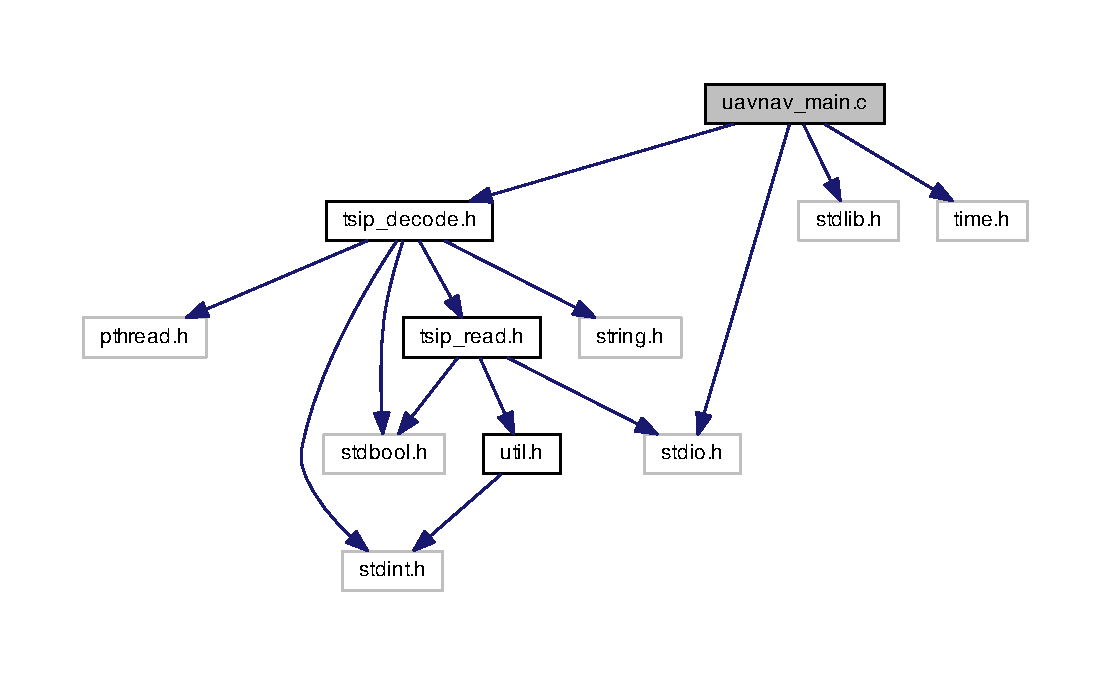
\includegraphics[width=350pt]{uavnav__main_8c__incl}
\end{center}
\end{figure}
\subsection*{Functions}
\begin{DoxyCompactItemize}
\item 
void \hyperlink{uavnav__main_8c_aad6066d9ede8cbf9b9d5e4fa28236380}{test\+\_\+data\+\_\+load} (const char $\ast$fname)
\begin{DoxyCompactList}\small\item\em Load a test data file. \end{DoxyCompactList}\item 
int \hyperlink{uavnav__main_8c_a0ddf1224851353fc92bfbff6f499fa97}{main} (int argc, char $\ast$argv\mbox{[}$\,$\mbox{]})
\begin{DoxyCompactList}\small\item\em Main function. \end{DoxyCompactList}\end{DoxyCompactItemize}
\subsection*{Variables}
\begin{DoxyCompactItemize}
\item 
unsigned char $\ast$ \hyperlink{uavnav__main_8c_a5e287a26406318ae22f91b2186e093a1}{g\+\_\+test\+\_\+data} = N\+U\+LL
\begin{DoxyCompactList}\small\item\em Test data array. \end{DoxyCompactList}\item 
uint32\+\_\+t \hyperlink{uavnav__main_8c_aa0982aa6ad6c582eac44366139eec768}{g\+\_\+test\+\_\+data\+\_\+len}
\begin{DoxyCompactList}\small\item\em Test data length. \end{DoxyCompactList}\item 
uint32\+\_\+t \hyperlink{uavnav__main_8c_af8a23b978deb1bf1c3e33bc838fecf69}{g\+\_\+test\+\_\+data\+\_\+start}
\begin{DoxyCompactList}\small\item\em Start of the test data. \end{DoxyCompactList}\item 
bool \hyperlink{uavnav__main_8c_af8fbc191e3a97ad0427003b79f03144e}{g\+\_\+verbose\+\_\+output}
\begin{DoxyCompactList}\small\item\em Verbose output parameter. \end{DoxyCompactList}\end{DoxyCompactItemize}


\subsection{Detailed Description}
Main tester application. Loads the test data files, runs tests, outputs the. 



\subsection{Function Documentation}
\mbox{\Hypertarget{uavnav__main_8c_a0ddf1224851353fc92bfbff6f499fa97}\label{uavnav__main_8c_a0ddf1224851353fc92bfbff6f499fa97}} 
\index{uavnav\+\_\+main.\+c@{uavnav\+\_\+main.\+c}!main@{main}}
\index{main@{main}!uavnav\+\_\+main.\+c@{uavnav\+\_\+main.\+c}}
\subsubsection{\texorpdfstring{main()}{main()}}
{\footnotesize\ttfamily int main (\begin{DoxyParamCaption}\item[{int}]{argc,  }\item[{char $\ast$}]{argv\mbox{[}$\,$\mbox{]} }\end{DoxyParamCaption})}



Main function. 

Loads a tester data file, runs tests.


\begin{DoxyParams}[1]{Parameters}
\mbox{\tt in}  & {\em argc} & Number of arguments. \\
\hline
\mbox{\tt in}  & {\em argv} & Arguments. \\
\hline
\end{DoxyParams}
\begin{DoxyReturn}{Returns}

\end{DoxyReturn}
\mbox{[}Loading a test file\mbox{]}

\mbox{[}Loading a test file\mbox{]} \mbox{[}Running a verbose test\mbox{]}

\mbox{[}Running a verbose test\mbox{]}

\mbox{[}Running a timed test\mbox{]}

\mbox{[}Running a timed test\mbox{]} \mbox{\Hypertarget{uavnav__main_8c_aad6066d9ede8cbf9b9d5e4fa28236380}\label{uavnav__main_8c_aad6066d9ede8cbf9b9d5e4fa28236380}} 
\index{uavnav\+\_\+main.\+c@{uavnav\+\_\+main.\+c}!test\+\_\+data\+\_\+load@{test\+\_\+data\+\_\+load}}
\index{test\+\_\+data\+\_\+load@{test\+\_\+data\+\_\+load}!uavnav\+\_\+main.\+c@{uavnav\+\_\+main.\+c}}
\subsubsection{\texorpdfstring{test\+\_\+data\+\_\+load()}{test\_data\_load()}}
{\footnotesize\ttfamily void test\+\_\+data\+\_\+load (\begin{DoxyParamCaption}\item[{const char $\ast$}]{fname }\end{DoxyParamCaption})}



Load a test data file. 

Loads a tester data file into workspace.


\begin{DoxyParams}[1]{Parameters}
\mbox{\tt in}  & {\em fname} & File name. \\
\hline
\end{DoxyParams}
\begin{DoxyReturn}{Returns}

\end{DoxyReturn}


\subsection{Variable Documentation}
\mbox{\Hypertarget{uavnav__main_8c_a5e287a26406318ae22f91b2186e093a1}\label{uavnav__main_8c_a5e287a26406318ae22f91b2186e093a1}} 
\index{uavnav\+\_\+main.\+c@{uavnav\+\_\+main.\+c}!g\+\_\+test\+\_\+data@{g\+\_\+test\+\_\+data}}
\index{g\+\_\+test\+\_\+data@{g\+\_\+test\+\_\+data}!uavnav\+\_\+main.\+c@{uavnav\+\_\+main.\+c}}
\subsubsection{\texorpdfstring{g\+\_\+test\+\_\+data}{g\_test\_data}}
{\footnotesize\ttfamily unsigned char$\ast$ g\+\_\+test\+\_\+data = N\+U\+LL}



Test data array. 

\mbox{\Hypertarget{uavnav__main_8c_aa0982aa6ad6c582eac44366139eec768}\label{uavnav__main_8c_aa0982aa6ad6c582eac44366139eec768}} 
\index{uavnav\+\_\+main.\+c@{uavnav\+\_\+main.\+c}!g\+\_\+test\+\_\+data\+\_\+len@{g\+\_\+test\+\_\+data\+\_\+len}}
\index{g\+\_\+test\+\_\+data\+\_\+len@{g\+\_\+test\+\_\+data\+\_\+len}!uavnav\+\_\+main.\+c@{uavnav\+\_\+main.\+c}}
\subsubsection{\texorpdfstring{g\+\_\+test\+\_\+data\+\_\+len}{g\_test\_data\_len}}
{\footnotesize\ttfamily uint32\+\_\+t g\+\_\+test\+\_\+data\+\_\+len}



Test data length. 

\mbox{\Hypertarget{uavnav__main_8c_af8a23b978deb1bf1c3e33bc838fecf69}\label{uavnav__main_8c_af8a23b978deb1bf1c3e33bc838fecf69}} 
\index{uavnav\+\_\+main.\+c@{uavnav\+\_\+main.\+c}!g\+\_\+test\+\_\+data\+\_\+start@{g\+\_\+test\+\_\+data\+\_\+start}}
\index{g\+\_\+test\+\_\+data\+\_\+start@{g\+\_\+test\+\_\+data\+\_\+start}!uavnav\+\_\+main.\+c@{uavnav\+\_\+main.\+c}}
\subsubsection{\texorpdfstring{g\+\_\+test\+\_\+data\+\_\+start}{g\_test\_data\_start}}
{\footnotesize\ttfamily uint32\+\_\+t g\+\_\+test\+\_\+data\+\_\+start}



Start of the test data. 

\mbox{\Hypertarget{uavnav__main_8c_af8fbc191e3a97ad0427003b79f03144e}\label{uavnav__main_8c_af8fbc191e3a97ad0427003b79f03144e}} 
\index{uavnav\+\_\+main.\+c@{uavnav\+\_\+main.\+c}!g\+\_\+verbose\+\_\+output@{g\+\_\+verbose\+\_\+output}}
\index{g\+\_\+verbose\+\_\+output@{g\+\_\+verbose\+\_\+output}!uavnav\+\_\+main.\+c@{uavnav\+\_\+main.\+c}}
\subsubsection{\texorpdfstring{g\+\_\+verbose\+\_\+output}{g\_verbose\_output}}
{\footnotesize\ttfamily bool g\+\_\+verbose\+\_\+output}



Verbose output parameter. 


\hypertarget{util_8h}{}\section{util.\+h File Reference}
\label{util_8h}\index{util.\+h@{util.\+h}}


Header containing the utility functions. Various utility functions, including the C\+RC checker.  


{\ttfamily \#include $<$stdint.\+h$>$}\newline
Include dependency graph for util.\+h\+:
\nopagebreak
\begin{figure}[H]
\begin{center}
\leavevmode
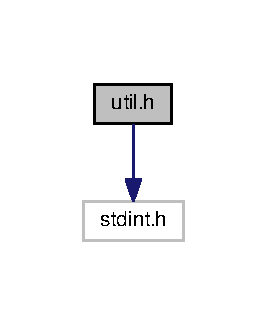
\includegraphics[width=128pt]{util_8h__incl}
\end{center}
\end{figure}
This graph shows which files directly or indirectly include this file\+:
\nopagebreak
\begin{figure}[H]
\begin{center}
\leavevmode
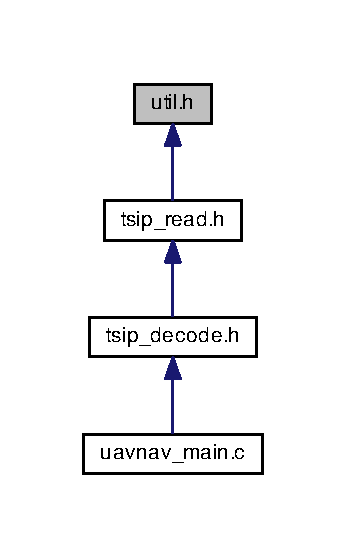
\includegraphics[width=166pt]{util_8h__dep__incl}
\end{center}
\end{figure}
\subsection*{Macros}
\begin{DoxyCompactItemize}
\item 
\#define \hyperlink{util_8h_affe776513b24d84b39af8ab0930fef7f}{max}(a,  b)
\item 
\#define \hyperlink{util_8h_ac6afabdc09a49a433ee19d8a9486056d}{min}(a,  b)
\end{DoxyCompactItemize}
\subsection*{Functions}
\begin{DoxyCompactItemize}
\item 
uint32\+\_\+t \hyperlink{util_8h_aa1921745f0c9cd9f201d624ca86dc40b}{crc32} (const uint8\+\_\+t $\ast$buf, const uint32\+\_\+t start, const uint32\+\_\+t end)
\begin{DoxyCompactList}\small\item\em C\+RC calculation for T\+S\+IP packets. \end{DoxyCompactList}\item 
uint32\+\_\+t \hyperlink{util_8h_ad96587305bb46bd47c2069e0aafd6530}{arr\+\_\+to\+\_\+int} (const uint8\+\_\+t $\ast$in, const uint32\+\_\+t n\+\_\+bytes)
\begin{DoxyCompactList}\small\item\em Convert an array of bytes into an integer for C\+RC check. \end{DoxyCompactList}\end{DoxyCompactItemize}
\subsection*{Variables}
\begin{DoxyCompactItemize}
\item 
const uint32\+\_\+t \hyperlink{util_8h_aaf584663e7fa9218e6f9f515ff41c6e4}{crc32\+\_\+table} \mbox{[}$\,$\mbox{]}
\begin{DoxyCompactList}\small\item\em Table of constants used for C\+RC calculation. \end{DoxyCompactList}\end{DoxyCompactItemize}


\subsection{Detailed Description}
Header containing the utility functions. Various utility functions, including the C\+RC checker. 



\subsection{Macro Definition Documentation}
\mbox{\Hypertarget{util_8h_affe776513b24d84b39af8ab0930fef7f}\label{util_8h_affe776513b24d84b39af8ab0930fef7f}} 
\index{util.\+h@{util.\+h}!max@{max}}
\index{max@{max}!util.\+h@{util.\+h}}
\subsubsection{\texorpdfstring{max}{max}}
{\footnotesize\ttfamily \#define max(\begin{DoxyParamCaption}\item[{}]{a,  }\item[{}]{b }\end{DoxyParamCaption})}

{\bfseries Value\+:}
\begin{DoxyCode}
(\{                                                                           \(\backslash\)
    \_\_typeof\_\_(a) \_a = (a);                                                    \(\backslash\)
    \_\_typeof\_\_(b) \_b = (b);                                                    \(\backslash\)
    \_a > \_b ? \_a : \_b;                                                         \(\backslash\)
  \})
\end{DoxyCode}
\mbox{\Hypertarget{util_8h_ac6afabdc09a49a433ee19d8a9486056d}\label{util_8h_ac6afabdc09a49a433ee19d8a9486056d}} 
\index{util.\+h@{util.\+h}!min@{min}}
\index{min@{min}!util.\+h@{util.\+h}}
\subsubsection{\texorpdfstring{min}{min}}
{\footnotesize\ttfamily \#define min(\begin{DoxyParamCaption}\item[{}]{a,  }\item[{}]{b }\end{DoxyParamCaption})}

{\bfseries Value\+:}
\begin{DoxyCode}
(\{                                                                           \(\backslash\)
    \_\_typeof\_\_(a) \_a = (a);                                                    \(\backslash\)
    \_\_typeof\_\_(b) \_b = (b);                                                    \(\backslash\)
    \_a < \_b ? \_a : \_b;                                                         \(\backslash\)
  \})
\end{DoxyCode}


\subsection{Function Documentation}
\mbox{\Hypertarget{util_8h_ad96587305bb46bd47c2069e0aafd6530}\label{util_8h_ad96587305bb46bd47c2069e0aafd6530}} 
\index{util.\+h@{util.\+h}!arr\+\_\+to\+\_\+int@{arr\+\_\+to\+\_\+int}}
\index{arr\+\_\+to\+\_\+int@{arr\+\_\+to\+\_\+int}!util.\+h@{util.\+h}}
\subsubsection{\texorpdfstring{arr\+\_\+to\+\_\+int()}{arr\_to\_int()}}
{\footnotesize\ttfamily uint32\+\_\+t arr\+\_\+to\+\_\+int (\begin{DoxyParamCaption}\item[{const uint8\+\_\+t $\ast$}]{in,  }\item[{const uint32\+\_\+t}]{n\+\_\+bytes }\end{DoxyParamCaption})}



Convert an array of bytes into an integer for C\+RC check. 


\begin{DoxyParams}{Parameters}
{\em in} & Pointer to array. \\
\hline
{\em n\+\_\+bytes} & Number of bytes to merge \\
\hline
\end{DoxyParams}
\begin{DoxyReturn}{Returns}
Calcutated integer . 
\end{DoxyReturn}
\mbox{\Hypertarget{util_8h_aa1921745f0c9cd9f201d624ca86dc40b}\label{util_8h_aa1921745f0c9cd9f201d624ca86dc40b}} 
\index{util.\+h@{util.\+h}!crc32@{crc32}}
\index{crc32@{crc32}!util.\+h@{util.\+h}}
\subsubsection{\texorpdfstring{crc32()}{crc32()}}
{\footnotesize\ttfamily uint32\+\_\+t crc32 (\begin{DoxyParamCaption}\item[{const uint8\+\_\+t $\ast$}]{buf,  }\item[{const uint32\+\_\+t}]{start,  }\item[{const uint32\+\_\+t}]{end }\end{DoxyParamCaption})}



C\+RC calculation for T\+S\+IP packets. 


\begin{DoxyParams}{Parameters}
{\em buf} & Pointer to buffer containing data to process. \\
\hline
{\em start} & Offset value of first data byte (within buf) to be processed. \\
\hline
{\em end} & Offset value of last data byte (within buf) to be processed. \\
\hline
\end{DoxyParams}
\begin{DoxyReturn}{Returns}
Calculated C\+RC value. 
\end{DoxyReturn}


\subsection{Variable Documentation}
\mbox{\Hypertarget{util_8h_aaf584663e7fa9218e6f9f515ff41c6e4}\label{util_8h_aaf584663e7fa9218e6f9f515ff41c6e4}} 
\index{util.\+h@{util.\+h}!crc32\+\_\+table@{crc32\+\_\+table}}
\index{crc32\+\_\+table@{crc32\+\_\+table}!util.\+h@{util.\+h}}
\subsubsection{\texorpdfstring{crc32\+\_\+table}{crc32\_table}}
{\footnotesize\ttfamily const uint32\+\_\+t crc32\+\_\+table\mbox{[}$\,$\mbox{]}}



Table of constants used for C\+RC calculation. 


%--- End generated contents ---

% Index
\backmatter
\newpage
\phantomsection
\clearemptydoublepage
\addcontentsline{toc}{chapter}{Index}
\printindex

\end{document}
